\subsection{Factoid \& List Type Questions}

% The key objective in extraction-based factoid and list type question answering systems is to find a subset of entities (or phrases) from the relevant snippets that are most likely to answer the question. 
Most of the state-of-the-art models for this task involve training end-to-end deep neural architectures to identify a subset of entities (or phrases) from the relevant snippets that are most likely to answer the question. But, owing to the small size of the dataset, we cannot effectively train such models on the BioASQ dataset. Hence, we adopted a two-stage approach that first finds a set  of entities that could potentially answer the question and a supervised classifier to rank the entities on the basis of their likelihood of answering the question.

For devising the model and evaluation, we primarily focused on factoid type questions since the methodology for the list-type question would be largely similar and different only in the number of top entities returned. 

\begin{table}[h]
    \centering
    \begin{tabular}{cccc} \hline
    \multirow{3}{*}{NER Tags} & 
    \multicolumn{2}{c}{\% of questions} & 
     \% of \\
    & Exactly & Partially & tokens \\
    & Answered & Answered & extracted \\ \hline
    PubTator & 32.05 &	72.15 & 52.27 \\
    Gram CNN & 34.90 &	99.03 & 94.97 \\
    LingPipe & 26.67 &	76.75 & 11.06 \\
    Union    & 49.04 &	99.65 & 99.25 \\
    Intersection & 16.29 &	38.00 & 3.33 \\ \hline
    \end{tabular}
    \caption{Baseline recall of different NER Taggers measured by the fraction of questions that can be answered by an ideal classifier if the candidates are chosen using the tagger. We also measure precision as the fraction of total unique tokens from the documents that are tagged.}
    \label{tab:NER_tagging_performances}
\end{table}

\begin{table*}[t!]
    \centering
    \begin{tabular}{|c|c|c|c|c|} 
    \hline \hline
    Model & Exact Answers & Exact Answers & Exact Answers & Ideal Answers \\
    &Yes/No type& Factoid  type& List type & All types \\
    & Accuracy (\%) & MRR & F1 score & ROUGE-2\\
    \hline \hline
    \cite{khyati-paper} & - & - & - & 0.653  \\
    \hline
    \cite{fudan}&\textbf{0.714}&0.272& 0.187& -\\
    \hline
    \cite{fastqa}& - &\textbf{0.392}& \textbf{0.361}&-\\
    \hline
    Sarrouti and Alaoui \shortcite{usmba}&0.461&0.207&0.243&0.577\\
    \hline
    \textit{BioAMA}(Ours)&0.653& 0.195&0.234&\textbf{0.721}\\
    \hline \hline
    
    \end{tabular}
    \caption{Comparison of our model with other state of the art approaches}
    \label{tab:comparison_results}
\end{table*}
\vspace{-0.3cm}
\subsubsection{Candidate Selection}

We found that the most critical step in the answer generation process is to identify the set of potential answer candidates that can be fed into a classifier or ranker to identify the best candidates. At first, in order to accomplish this, we used Named Entity Recognition (NER) taggers to form a set of candidate answers. The taggers that we used include Gram-CNN \cite{gram-cnn}, LingPipe\cite{lingpipe} and PubTator \cite{pubtator}. To analyze the effectiveness of these taggers, we performed an analysis on BioASQ training set 5b by evaluating the fraction of questions whose answers are included in the candidate entity set by the taggers.

Table \ref{tab:NER_tagging_performances} shows the relative performances of the three taggers, their union as well as intersection on train dataset of BioASQ 5b factoid type questions. A question is exactly answered if a tagger tags an entity that matches an answer exactly, and it is partially answered if there is a non-zero overlap with an entity tagged and an answer for the question. We can notice that PubTator and LingPipe have a good recall with relatively low precision, while Gram CNN has high recall but low precision. However, the final results with the Named Entity Taggers were not aligned with our expectations. This is mostly because the answers for BioASQ are usually a combination of BioNERs and complementary words, making it hard to define a pruning method that is able to yield satisfactory results. Surprisingly, a group of candidates formed of the 100 most frequent \texti{n}-grams (\textit{n} from 1 to 4) from the snippets' sentences were a better candidate group than the NER approach for our supervised ranking method and we decided to use the NER taggers as features instead of candidate groups.


\subsubsection{Classification Features}\label{sec:classification_features}

Upon computing the set of candidate answers, we use the question $q$, set of relevant snippet sentences $\mathcal{S}$ and entity type $t_i$ to devise a feature vector for each individual entity $e_i$ that comprises the following features:

\begin{itemize}[noitemsep]
    \item BM25 Score: The BM25 scores for all the sentences are computed with the question as the query. Then, the scores of the sentence that contain the entity are aggregated to compute the BM25 score for the entity, i.e.
    \begin{align*}
    %     \text{BM25 }&\text{Score($e_i$)} \\
    %   &= \sum_{s \in \mathcal{S}} \text{BM25 Score($e_i$)} \cdot \mathbbm{1}(s, e_i)
        \text{Score}_{BM25}(e_i) &= \sum_{s \in \mathcal{S}} \text{Score}_{BM25}(e_i) \cdot \mathbbm{1}(s, e_i)
    \end{align*}
    where $\mathbbm{1}(s, e_i)$ is 1 iff sentence $s$ has entity $e_i$.
    \item Indri Score: Computed in the same manner as BM25 score in (i)
    \item Number of Sentences: Number of sentences $s \in \mathcal{S}$ that contain the entity $e_i$
    \item NER Tagger: A multinomial feature that represents which tagger among PubTator, LingPipe and GramCNN the entity was extracted with. This feature is included to identify the relative strengths of the different taggers.
    \item Tf Idf: The aggregate Tf-Idf scores of the entity with $\mathcal{S}$ as the set of documents
    \item Entity Type: Is a boolean feature that is 1 if the type of the entity (for example, \textit{gene}) is present in the question, and 0 otherwise.
    \item Relative Frequency: The amount of times the entity appears on the snippets' sentences divided by the total appearance of all of the relevant entities.
    \item Query Presence: Is a boolean feature that is 1 if the query contains the entity completely and 0 otherwise.

\end{itemize}

\subsubsection{Unsupervised Ranking}

As a baseline, we first present an unsupervised ranking system for the candidate answers. In this system, the snippet sentences are first ranked using the BM25 model. Then, for each entity, a score is computed by aggregating the BM25 scores of the sentences in which the entity is present. The rationale for this is that the entities in the top ranked sentences are more likely to be the answers. This entity score (which is equivalent to the BM25 score described in \ref{sec:classification_features}) is then used to rank the entities and return the top $k$ entities as answers to the question. The overall unsupervised system is shown in Figure \ref{fig:UnsupervisedNERPipeline}.

\begin{figure}
    \centering
    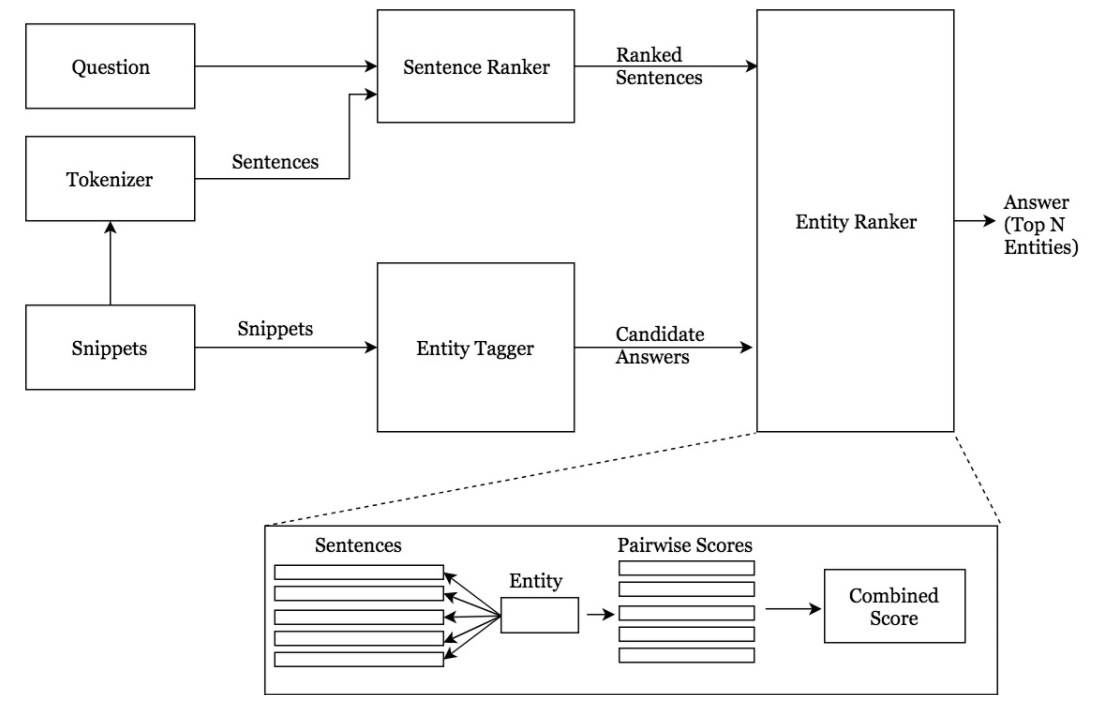
\includegraphics[scale=0.4]{UnsupervisedNERPipeline.png}
    \caption{Unsupervised generation of factoid/list type answers using NER taggers and BM25 retrieval model}
    \label{fig:UnsupervisedNERPipeline}
\end{figure}

\subsubsection{Learning To Rank}

In order to rank the candidate entities in a supervised way, we used a ranking classifier based on the features described in \ref{sec:classification_features}. For ranking, we chose point-wise ranking classifiers over pair-wise and list-wise, because it yields similar results to ranking methods with a less time-consuming and computationally expensive approach. We are using a traditional SVM-Light \cite{svmlight} implementation for point-wise ranking. The data for supervision was derived from the actual answers and candidate entities were ranked based on their overlap with the actual answers. 

% and the model was trained to learn these rankings.

% The idea behind our approach for factoid and list types of questions are based on pairwise Learning To Rank (LeToR). Each questions consists of a group of snippets and the actual query body. Given a Candidates Space (C) of possible named entities, a query (q) and a group of sentences extracted from the snippets (S); our approach is to train a model which ranks each candidate c of C given S and q. Basically, we are learning a function $g(c_i,c_k,S,q)$ that incorporates a score for each pair ($c_i,c_k$) of the Candidates Space. With the respective rankings, we can create a ranked list of entities to be returned. Therefore, in order to execute the model, it's necessary to define a Candidates Space C; a feature vector for each combination $f(c_i,S,q)$; and a function g for $g(c_i,c_k,S,q)$.

Once we rank the entities, we use a naive approach of merely taking top 5 entities as answers for factoid type and top 10 for list-type. One could, however, devise a separate model for identifying the number of top entities to return as answers for the list-type answers. 

We found that using just the NER entities as the answer candidates, the classifier could achieve an MRR of 0.06 on factoid type questions and an F-measure of 0.18 for list type questions. However, by having all the n-grams ($n = 1, 2, 3, 4$) from the snippets as candidate answers and using NER tags as LeToR features, the performance was improved to an MRR of 0.195 on Factoid type questions and an F1 score of 0.234  on List type questions. The results are summarized in Table \ref{tab:comparison_results}.


% \newline \textbf{Features}: For features, we have used combination of syntactic, information retrieval, information theory, semantic and lexical features. POS tags, frequency, tf-idf, NER tags are examples of the features extracted for each candidate representation, which would consist of a vector of values between 0 and 1.  Therefore, for each candidate answer c for a question, we have a vector $v = f(c_i,S,q)$ that represents the features for this candidate.

% By directly testing and combining results, we decided to use the union of PubTator and LingPipe entities to build our Candidate Space. However, this was an insufficient approach due to the fact that it was too narrow to actually achieve reasonable results. Although the features chosen and the ranking model worked well, there was an upper bound precision available by this approach. Therefore, we shifted for different approaches: Noun's combinations, entity recognition systems not related to the biological domain and noun phrases. Noun Phrases have shown the best results: they are a large enough space (it doesn't create a hard bound limit for our results), but still possible to search and rank.

%\subsubsection{Results}
%The results of our list and factoid type questions are presented in Table \ref{tab:comparison_results}.

%\begin{table}[t!]
%    \centering
%    \begin{tabular}{ccc} \hline
%    Entities & Soft Accuracy (\%) & MRR (\%) \\ \hline
%    Pubtator & \textbf{7.14} & 3.35 \\
%    Lingpipe & 4.58 & 2.70 \\
%    Gram CNN & 0.98 & 0.24 \\
%    Union    & 1.05 & 0.38 \\
%    Intersection & 4.91 & \textbf{3.68} \\ \hline
%    \end{tabular}
%    \caption{Performance of unsupervised ranking model to identify the entities among the candidates from different taggers, for factoid type questions in BioASQ 5b dataset}
%    \label{tab:my_label}
%\end{table}

% Model	Exact Matches	Soft Matches	MRR Exact
% Pubtator	7.14%	50.71%	3.35%
% Lingpipe	4.58%	60.72%	2.70%
% Gram CNN	0.98%	85.53%	0.24%
% Ensemble Union	1.05%	85.29%	0.38%
% Ensemble Intersection	4.91%	39.47%	3.68%

